\chapter{Pedestal Modeling and Theory}\label{ch:Modeling}

While a number of high-performance regimes (described in \cref{ch:HighPerformance}) have been established and are actively explored for tokamak operation, much of the physics governing these regimes is still unknown.  In particular, the physics underlying the structure of the pedestal is an area of active research, due in large part to the inherent difficulty in experimentally diagnosing the pedestal plasma as it varies over short scale lengths, and in the wide variability of H-mode behaviors observed in tokamak experiments.  Nevertheless confidence in the prediction of pedestal height and stability for ITER- and reactor-scale devices is essential: core temperature and pressure in the plasma are strongly sensitive to pedestal conditions due to profile stiffness driven by marginally-stable temperature-gradient modes \cite{Hubbard1998}\gnote{elaborate or reword}, thus fusion power density is controlled by the pressure pedestal structure.  Moreover, operation with large, uncontrolled Edge-Localized Modes (ELMs -
- see \cref{sec:hcr_elmy}) can drive transient heat loads exceeding wall material tolerances on ITER-scale devices \cite{Loarte2003,Federici2003} -- an understanding of pedestal stability against ELMs is necessary for ITER operation and beyond.  This chapter provides a review of the efforts to date in theory and modeling of the pedestal, including the theoretical models used in the balance of this thesis.\nicesectionending\gnote{elaborate?}

\section{Early Models}\label{sec:mod_early}

\gnote{needs better title...}Initial efforts in understanding the pedestal took a variety of approaches, including models built from fairly simple \emph{ans\"{a}tze} for the physics determining the pedestal structure.  Several of these approaches are detailed here.  Overviews of these models may also be found in \cite[\S 2]{Hubbard2000,Hughes2005}.

\subsection{Empirical Observations}\label{subsec:mod_empirical}

Absent a firm understanding of the physics underlying the pedestal structure, experimental efforts have sought to characterize the pedestal in terms of simple scalings with engineering parameters.  The pedestal width, in particular, presented significant difficulty in this regard, as it tends to be quite robust, varying only over a narrow range on a given machine \cite{Maggi2010} -- observations on JET \cite{Breger1998} and Alcator C-Mod \cite{Hughes2002,Hughes2007a} found minimal variation of the pedestal width with plasma current or magnetic field, although a somewhat broader pedestal was observed at low current and with strong shaping on C-Mod \cite{Hughes2007,Hughes2007a}.  Accordingly, the measured gradients in density, temperature, and pressure in the steepest region of the pedestal trend linearly with the corresponding value at the pedestal top \cite{Breger1998,Hughes2007a}.

Multivariate dependences on engineering parameters may be explored with a reasonably general approach via power-law scalings, fitting pedestal data to scalings agnostic of any assumed underlying physics.  Suttrop \emph{et al.} \cite{Suttrop1997} found for ASDEX Upgrade pedestals

\begin{equation}
 \nabla p \sim B_T^{-0.31} \; P_{tot}^{0.16} \; \overline{n}_e^{-0.1} \; I_p^{2.1}
\end{equation}

\noindent A similar approach on C-Mod using an extensive dataset of EDA and ELM-free H-modes \cite{Hughes2002} found

\begin{equation}\label{eq:pedfits}
 \begin{aligned}
  n_{e,ped} &\sim I_p^{0.95} \; \overline{n}_{e,L}^{0.39} \; B_T^{-0.46}\\
  T_{e,ped} &\sim I_p^{0.95} \; \overline{n}_{e,L}^{-0.78} \; B_T^{0.80} \; P_{net}^{0.64}\\
  p_{e,ped} &\sim I_p^{1.98} \; \overline{n}_{e,L}^{-0.56} \; P_{net}^{0.48}
 \end{aligned}
\end{equation}

\noindent (here $\overline{n}_{e,L}$ is the L-mode target density, as pedestal density is not readily controllable in EDA H-mode).  However, later studies asserted that the magnetic-field dependence was overstated in the above \cite{Hughes2006}.  While these empirical models perform reasonably well on their respective experimental data, confident extrapolation to ITER-scale operation requires a physics-based understanding of the pedestal structure.

\subsection{Neutral Penetration \& the Density Pedestal}\label{subsec:mod_neutral}

Given the proximity of the plasma pedestal to neutral gas from fueling apparatus and wall outgassing in the edge, it is logical that the density profile should depend strongly on interaction with and ionization of neutral particles in the pedestal.  Based on a relatively simple particle transport model, the pedestal width is expected to scale with the characteristic neutral penetration length before ionization \cite{Hughes2005,Mahdavi2002}:

\begin{equation}\label{eq:neutralpenetration}
 \lambda_{neutral} = \frac{v_n}{n_e \langle \sigma v \rangle_{ion}}
\end{equation}

\noindent where $v_n$ is the velocity of neutrals entering the pedestal (set by the neutral thermal temperature in the edge) and $\langle \sigma v \rangle_{ion}$ is the velocity-averaged ionization cross-section.  Given that $v_n$ is independent of plasma conditions and that $\langle \sigma v \rangle_{ion}$ is consistent over the temperatures of interest in the edge \cite{Hughes2005}, therefore we expect the simple relation $\Delta_{n} \sim 1/n_{e,ped}$.  More complex models for the neutral penetration typically reproduce the dependence on $\lambda_{neutral}$.

However, experimental observations of the density pedestal conflict with these relatively simple predictions.    Observations in similarity experiments between DIII-D, JET, and ASDEX Upgrade \cite{Beurskens2011} were inconsistent with the simple model: although DIII-D data were consistent with the trends found in the model, data from JET were not, and moreover the model predicted an inconsistent scaling between the two machines for pedestal density and width.  Likewise, predictions based on pedestal widths set by neutral penetration performed poorly as a predictor for pedestal height in a multi-machine scaling from AUG, DIII-D, JT-60U, and JET \cite{Onjun2002}.  EDA H-modes on Alcator C-Mod show near-complete insensitivity of the density pedestal to neutral interactions -- the density pedestal instead saturates to a level dictated by plasma transport (predicted best by $n_{e,ped} \sim I_p$), with fueling via edge gas puffing having little effect on the density pedestal \cite{Hughes2006,Hughes2007}.

In addition to significant sensitivity to machine and discharge conditions and wall materials \cite{Beurskens2011}, density pedestal behavior appears to be strongly sensitive to magnetic configuration -- experiments on MAST \cite{Maggi2010} found that, while the density pedestal width was poloidally constant in single-null discharges, the density pedestal is measurably broader on the outboard, low-field side in double-null discharges.  These results indicate that plasma-neutral interactions in the density pedestal are quite complex, and dependent on poloidal transport behaviors and fueling asymmetries \cite{Maggi2010}.  This remains an important area of research, as ITER is expected to have an edge that is highly opaque to neutrals, complicating the density pedestal structure and fueling scenarios for high-density plasmas \cite{Hughes2007,Maggi2010}.

\subsection{Ion-Orbit Loss \& Gyroradius Models}\label{subsec:mod_ionorbitloss}

Due to the importance in the edge $E_r$ well in pedestal formation, modeling efforts naturally turned to potential sources for the electric field to explain the pedestal.  One suggested source was ion orbit loss across the last closed flux surface, in which the gyro-motion of ions near the edge intersect the SOL or the plasma-facing material surfaces -- the charge imbalance induced by this particle ``leak'' results in a radial electric field \cite{Shaing1990}.  Assuming ion orbit losses drive the $E_r$ well, the $\vec{E}\times\vec{B}$ shear layer width ought to be governed by the banana orbit width, which scales as the poloidal gyroradius $\rho_{i,pol} \sim \sqrt{T_i}/B_p$.  Accounting for the squeezing effect of the radial electric field on the banana orbit width, Shaing \cite{Shaing1992} gives for the well width

\begin{equation}\label{eq:Shaing_width}
 \begin{aligned}
  &\Delta_{\vec{E}\times\vec{B}} \propto \sqrt{\varepsilon} \frac{\rho_{i,pol}}{\sqrt{S}}\\
  &S = \left| 1 - \frac{1}{B_p \omega_{ci,p}} \frac{dE_r}{dr}\right|
 \end{aligned}
\end{equation}

\noindent where $S$ is the squeezing factor and $\omega_{ci,p}$ is the ion cyclotron frequency evaluated with the poloidal field.  The model is further refined by Itoh \& Itoh \cite{Itoh1996} to include the broadening effects of viscosity shear.  The predicted trend is observed in ELM-free H-modes on JT-60U \cite{Hatae1998}, with $\Delta \approx 3.3 \sqrt{\varepsilon} \rho_{i,pol}$; however, as the squeezing factor $S$ is estimated to be near-unity, the pedestal width is broader by a factor of $\sim 3.3$ than the $\sim \sqrt{\varepsilon} \rho_{i,pol}$ banana width.  ELMy H-modes on JT-60U exhibit a similar scaling at weak shaping, with a broader pedestal and additional safety factor dependence $\Delta \approx 5 \rho_{i,pol} q_{95}^{-0.3}$ at higher triangularity \cite{Kamada1999}.

However, other predictions and experimental observations contradict these results.  Depending on the calculation method of growth rate suppression by $\vec{E}\times\vec{B}$ sheared flow, the pedestal width may scale with the gyroradius anywhere from $\Delta \sim \left(\rho^*\right)^{1/2}$ to $\Delta \sim \rho^*$, where $\rho^*$ indicates the gyroradius normalized to the plasma minor radius \cite{Onjun2002,Beurskens2011}.  Alternately, stabilization of drift-ballooning modes leads to a predicted dependence of $\Delta \sim \rho_{i,pol}^{2/3}$ \cite{Wilson1997}; similarly, diamagnetic stabilization in the pedestal leads to the prediction of $\Delta \sim I_p^2 \rho_{i,pol}^{2/3}$ \cite{Rogers1999}.  Observations on DIII-D \cite{Osborne1998} found a dependence of $\Delta/R \sim (\rho_{i,pol}/R)^{0.67}$, while observations on ASDEX Upgrade \cite{Beurskens2011,Suttrop2000a} found no gyroradius dependence for the pedestal width.

Distinguishing between these scalings is difficult given the diagnostic complications inherent in pedestal measurements, and the narrow range over which $\rho_i$ or the pedestal and $E_r$ well width vary on a given machine \cite{Gohil1998,Maggi2010}.  Moreover, alternate models propose a scaling with poloidal beta at the pedestal top, rather than poloidal gyroradius, with trends of width of $\Delta \sim \beta_{p,ped}^{0.4}$ to $\sim \beta_{p,ped}^{0.5}$ observed on DIII-D \cite{Osborne1998,Groebner1998a}, JET \cite{Maggi2010}, JT=60U \cite{Urano2008}, and ASDEX Upgrade \cite{Beurskens2011}.  Due to the strong covariance between $\rho_{i,pol} \sim \sqrt{mT}/I_p$ and $\sqrt{\beta_{p,ped}} \sim \sqrt{nT}/I_p$ these trends are quite difficult to separate.  However, dedicated experiments to separate the two, either via pumping to vary density and temperature at fixed pressure, exploiting the density dependence in $\beta_{p,ped}$ \cite{Osborne1998}, or via isotope variation targeting the mass dependence in $\rho_{
i,pol}$ \cite{Urano2008,Saibene1999}, found the $\beta_{p,ped}$ scaling to be the better predictor, with a weaker secondary gyroradius dependence $\Delta \sim \rho_{i,pol}^{0.2} \beta_{p,ped}^{0.5}$ \cite{Urano2008,Maggi2010}.  The physics underlying the $\Delta \sim \sqrt{\beta_{p,ped}}$ scaling will be discussed in detail in \cref{sec:mod_turbulence}.\nicesectionending

\section{MHD Stability: Peeling-Ballooning Modes}\label{sec:mod_pb}

Due to the extremely rapid onset of explosive ELM instabilities, ideal MHD modes were identified early on as candidates for the ELM trigger \cite{Wagner1982,Keilhacker1984,Huysmans2005}.  In this section, we detail the development of models for the pedestal structure based on the idea that ELM instabilities represent an ultimate limit on the pedestal.

The stability of a plasma may be assessed via a linear perturbation to the customary MHD equations.  We consider a first-order perturbation $\vec{\xi}$ to a plasma fluid element -- typically the perturbation is considered general in spatial variables, and is taken to be a Fourier harmonic in time, $\vec{\xi} = \vec{\xi}(\psi,\chi,\zeta) \mbox{exp}(i\omega t)$ where $\psi$ is the flux coordinate, $\chi$ is the poloidal angle, and $\zeta$ is the  toroidal angle.  Substituting into the first-order perturbation of the MHD equations\gnote{detail these in intro?} results in the simple relation (see \cite[\S 8]{Freidberg1987} for derivation)

\begin{equation}\label{eq:mhd_perturb}
 \rho \frac{d^2 \vec{xi}}{dt^2} = -\omega^2 \rho \vec{\xi} = \vec{F}(\vec{\xi})
\end{equation}

\noindent where $\omega$ is the mode frequency, $\rho$ is the mass density, and $\vec{F}$ is a forcing operator given by

\begin{equation}\label{eq:forcing}
 \begin{aligned}
  \vec{F}(\vec{\xi}) &= \frac{1}{\mu_0} \left( \nabla \times \vec{B} \right) \times \vec{Q} + \frac{1}{\mu_0} \left( \nabla \times \vec{Q} \right) \times \vec{B} + \nabla \left( \vec{\xi} \cdot \nabla p + \gamma p \nabla \cdot \vec{\xi} \right)\\
  \vec{Q} &= \nabla \times \left( \vec{\xi} \times \vec{B} \right)
 \end{aligned}
\end{equation}

\noindent with $\vec{Q}$ for the perturbed magnetic field and $\gamma$ for the specific heat ratio of the plasma.  The usual treatment of this operator leverages the fact that $\vec{F}$ is self-adjoint (\ie it is its own complex conjugate) -- this permits by integration over the plasma volume $P$ in a variational formulation

\begin{equation}\label{eq:energyprinciple}
 \begin{aligned}
  \omega^2 &= \frac{\delta W(\vec{\xi}^*,\vec{\xi})}{K(\vec{\xi}^*,\vec{\xi})}\\
  \delta W &= -\frac{1}{2} \int_P \vec{\xi}^* \cdot \vec{F}(\vec{\xi}) \;d^3 \vec{r}\\
  K &= \frac{1}{2} \int_P \rho \left| \vec{\xi} \right|^2 \;d^3 \vec{r}
 \end{aligned}
\end{equation}

\noindent This formulation permits the use of the \emph{energy principle}: if the potential energy $\delta W$ is negative for any displacement (\ie the perturbation drives the plasma to a more energetically-favorable state) then the mode corresponding to that displacement is unstable, captured by the fact that $\delta W < 0$ requires an imaginary frequency $\omega$ (and thus will have an exponentially growing mode).  

This permits a conceptually straightforward means to assess mode stability.  However, the formulation for $\delta W$ is highly involved (see \cite[\S 8.8]{Freidberg1987}):

\begin{equation}\label{eq:deltaW}
 \begin{aligned}
  \delta W &= \delta W_F + \delta W_S + \delta W_V\\
  \delta W_F &= \frac{1}{2} \int_P d^3 \vec{r} \Bigg[ \frac{|\vec{Q}|^2}{\mu_0} + \frac{B^2}{\mu_0} \left| \nabla \cdot \vec{\xi}_\perp + 2 \vec{\xi}_\perp \cdot \vec{\kappa} \right|^2 + \gamma p \left| \nabla \cdot \vec{\xi} \right|^2\\
  &\quad- 2\left( \vec{\xi}_\perp \cdot \nabla p \right) \left(\vec{\kappa} \cdot \vec{\xi}_\perp^* \right) - j_\parallel \left(\vec{\xi}_\perp^* \times \vec{b} \right) \cdot \vec{Q}_\perp \Bigg]\\
  \delta W_S &= \frac{1}{2} \int_S dS \left| \hat{n} \cdot \vec{\xi}_\perp \right|^2 \hat{n} \cdot \left[ \nabla \left( p + \frac{B^2}{2\mu_0} \right) \right]\\
  \delta W_V &= \frac{1}{2} \int_V d^3 \vec{r} \frac{\left|B_1 \right|^2}{\mu_0}
 \end{aligned}
\end{equation}

\noindent for the fluid, surface, and vacuum energy contributions integrated over the plasma volume $P$, plasma surface $S$, and vacuum volume $V$ respectively (in the above $\vec{\kappa}$ is the vectorized curvature, $\hat{n}$ is the normal vector to the plasma surface, and $B_1$ is the perturbed magnetic field in the vacuum region).  The complexity of the stability problem necessitates both a firm theoretical understanding to simplify \cref{eq:deltaW} to a tractable form, and numerical approaches to efficiently calculate the stability in experimental plasmas.

\subsection{Ballooning MHD}\label{subsec:mod_balloon}

Examining the fluid energy formulation $\delta W_F$ in \cref{eq:deltaW}, we see two potential sources of instability (that is, negative terms in $\delta W$) -- these identify the pressure gradient $\nabla p$ and the parallel current density $j_\parallel$ as potential sources of free energy to drive unstable modes.

\begin{itemize}
 \item early observations of pressure gradient limit at ELM trigger \cite{Kamada1996,Suttrop2000}
 \item value of pressure gradient at limit increases with $I_p$, shaping \cite{Suttrop2000a}
 \item measured $\alpha_{MHD}$ exceeds stable prediction by BALOO in DIII-D ELMy H-modes -- need to account for current, finite-$n$ effects \cite{Groebner1998a,Osborne1998}
 \item EDA H-mode modeled to be ideal-ballooning stable; P-B only describes ELMy H-mode \cite{Mossessian2002}
 \item increased triangularity reduces $\nabla p$, $n_{e,ped}$ in EDA; contrast with ELMy, where shape stabilizes P-B modes, seems to destabilize QCM earlier in EDA \cite{Hughes2007a}
 \item DIII-D VH-modes terminate in giant p-b driven ELM \cite{Turnbull2003}
\end{itemize}

\subsection{Peeling MHD}\label{subsec:mod_peel}

\subsection{ELITE Code}\label{subsec:mod_elite}

\begin{itemize}
 \item strong shaping impacts stability contour in $j-\alpha_{MHD}$ space \cite{Snyder2009}
 \item collisionality $\rightarrow$ bootstrap current $\rightarrow$ magnetic shear in edge sets where in stability contour pedestal hits \cite{Snyder2009}
 \item due to interplay, nonlocal effects between shaping, collisionality, rotation, shafranov shift, safety factor, must calculate P-B stability in 2D: can't reduce to scalar parametrization \cite{Snyder2009}
 \item Snyder2009 refs Huysmans2005, Turnbull2003, Medvedev2006 \cite{Huysmans2005,Turnbull2003,Medvedev2006} for reviews of alternate MHD codes
 \item alternate MHD codes: GATO \cite{Bernard1981}, MISHKA \cite{Huysmans2001,Mikhailovskii1997}, KINX \cite{Degtyarev1997,Medvedev2006}, MARG2D \cite{Aiba2006,Aiba2007}
 \item RMP approaches P-B boundary, EDA, type-III ELMs P-B stable, grassy/type-II ELMs near boundary, QH near low-$n$ peeling side -- P-B boundary figure of merit in general for H-mode pedestal \cite{Snyder2009}.  RMP calcs stable, goes ELMing and crosses boundary as soon as coils are turned off \cite{Snyder2009a}
 \item very low $n$ ($n < 3$) modes omitted from ELITE: low-$n$ edge modes rarely more unstable than $n \sim 5$, code cannot distinguish from core kink modes, low-$n$ modes stabilized by interaction with wall \cite{Snyder2009}
 \item ELITE omits X-point from calculation due to required extremely high RZ point density; peeling modes highly unstable there, but high collisionality at LCFS suppresses.  Calculation usually truncated at 99.8\% flux \cite{Snyder2009a}
 \item check Snyder2009a for ELITE alternate refs; Huysmans2005, Wilson2006 for reviews \cite{Snyder2009a,Huysmans2005,Wilson2006}
\end{itemize}

\begin{figure}
 \pushtooutside
 \ffigbox[\FBwidth]{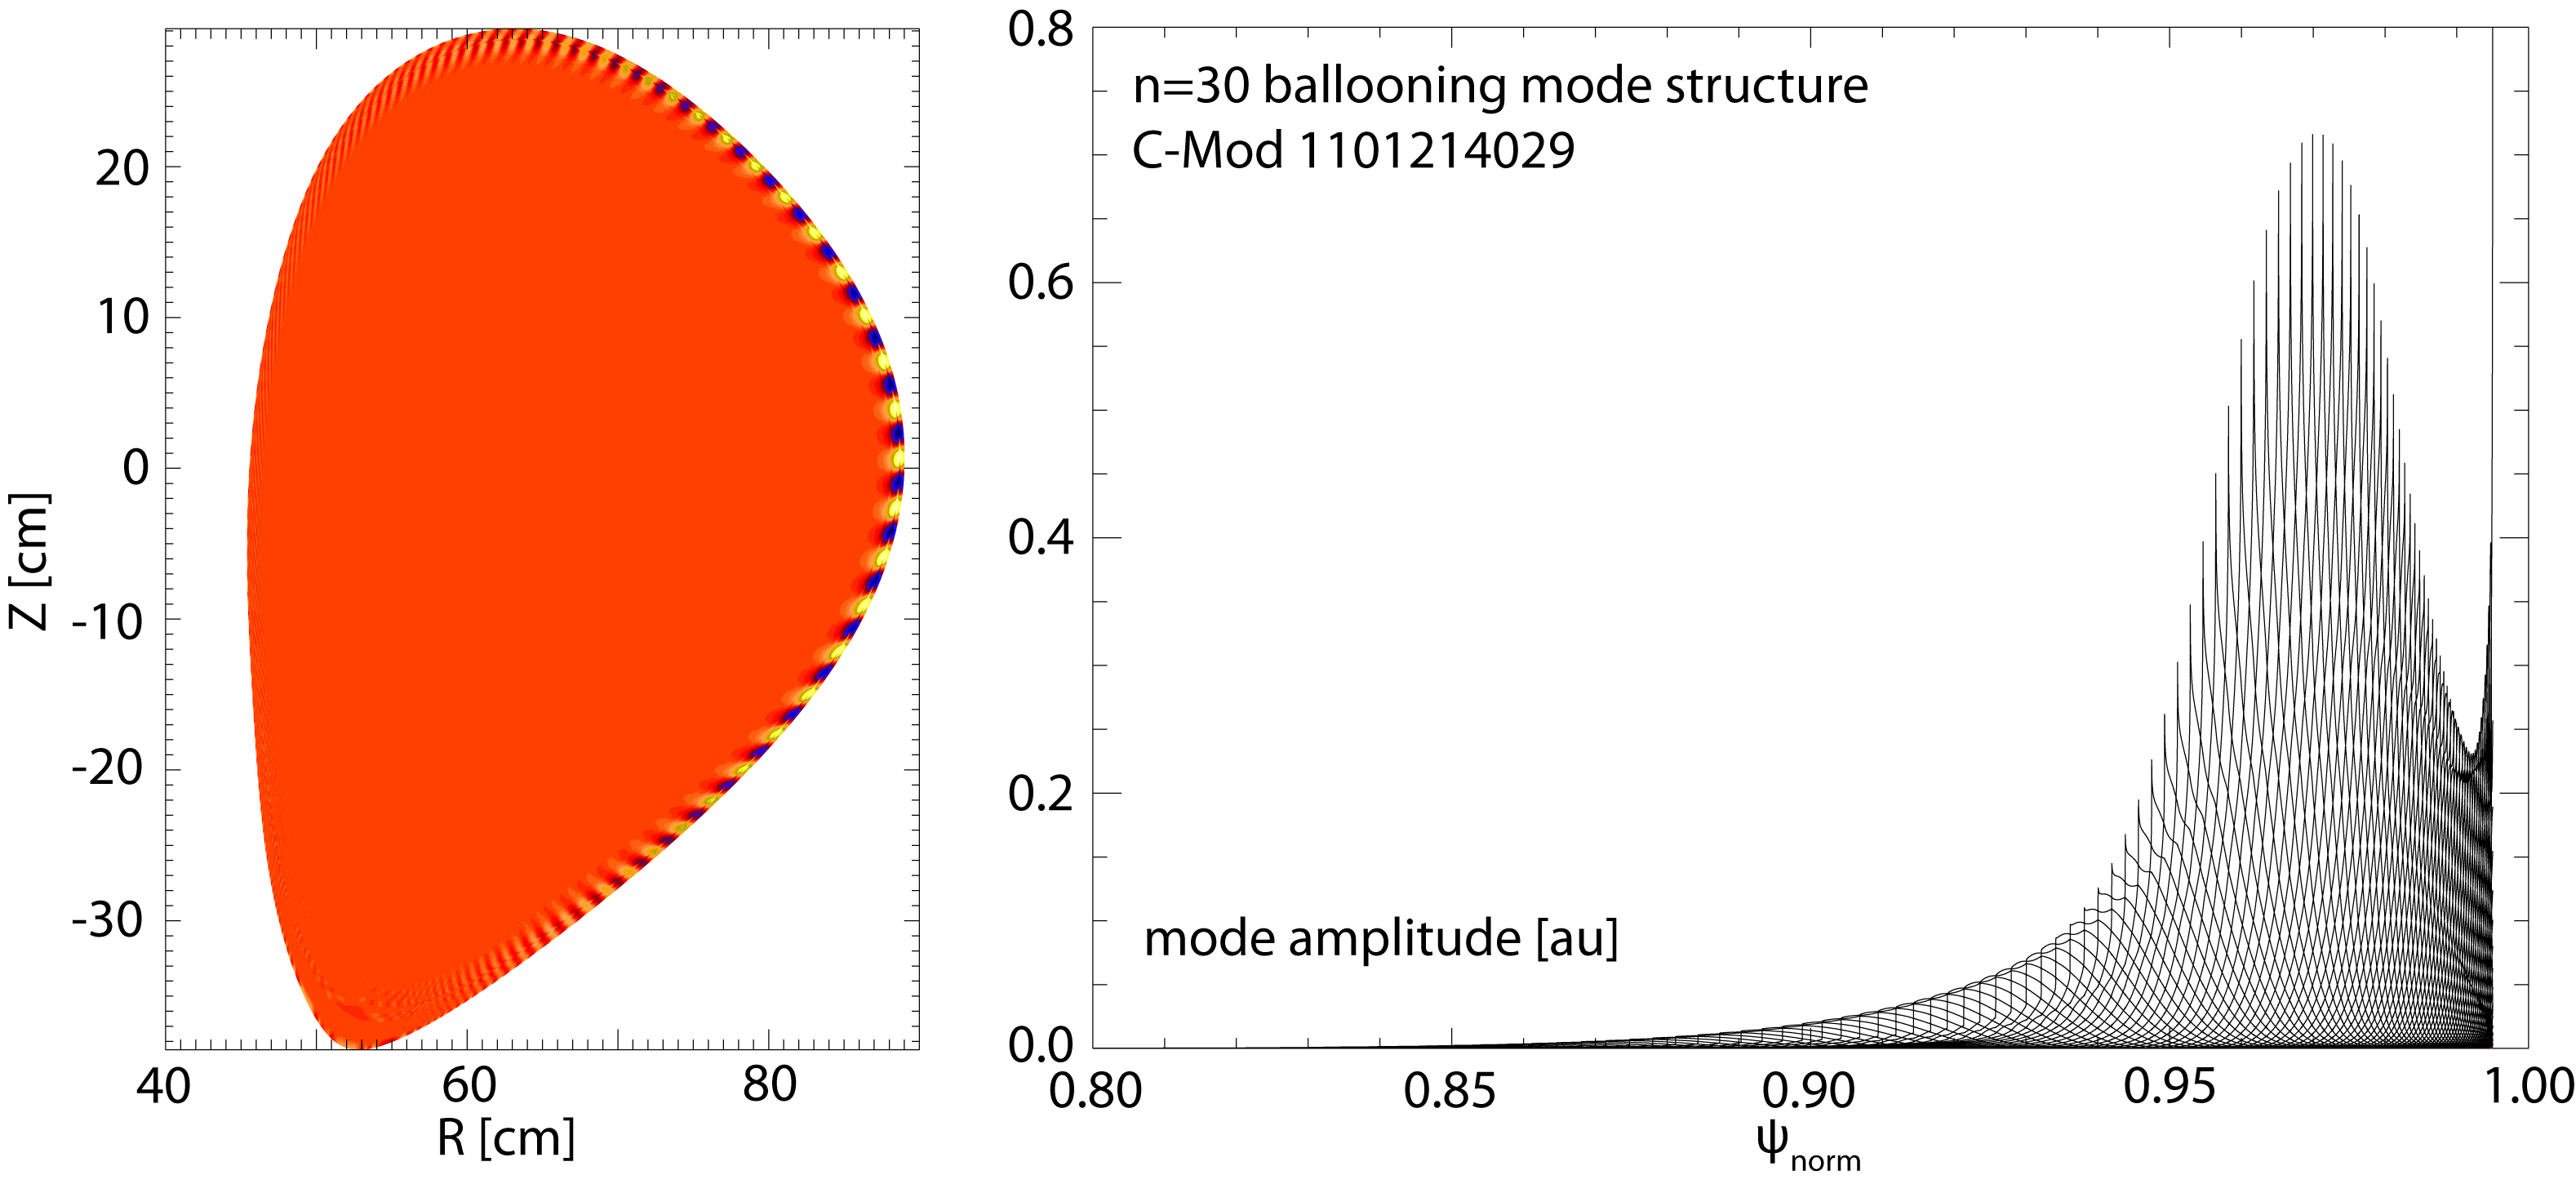
\includegraphics[width=150mm]{graphics/ModelingTheory/pb_modestructure.pdf}}{\caption[Mode structure for $n=30$ model calculated by ELITE.]{Mode structure for an $n=30$ ballooning mode calculated by ELITE.  (left) Contour plot of radial perturbations from the mode.  The mode is edge-localized and strongest at the outboard midplane, consistent with an edge ballooning mode.  (right) Eigenmode structure of the $n=30$ mode.  Each peak is a poloidal harmonic localized around the rational flux surface determined by the corresponding poloidal mode number $m$ for $n=30$.  The mode is strongest in the steep gradient region, but extends inward due to the comparatively high mode number (eigenmode envelope encompasses $O(n^{1/3})$ flux surfaces).  Note that, as ELITE cannot treat the separatrix, the mode calculation truncates at $\psi_{norm} = 0.995$.}\label{fig:pb_modestructure}}
\end{figure}

\begin{figure}
 \pushtooutside
 \fcapside[60mm]{\caption[Schematic of peeling-ballooning MHD stability space.]{Schematic of the stability space to coupled peeling-ballooning MHD modes, set by the edge pressure gradient and current density.  Ballooning modes are driven by pressure gradient but stabilized by magnetic shear driven by edge currents, while kink/peeling modes are current-driven but stabilized by pressure gradients.  \note{Ref to Snyder?}}\label{fig:mod_pbcartoon}}{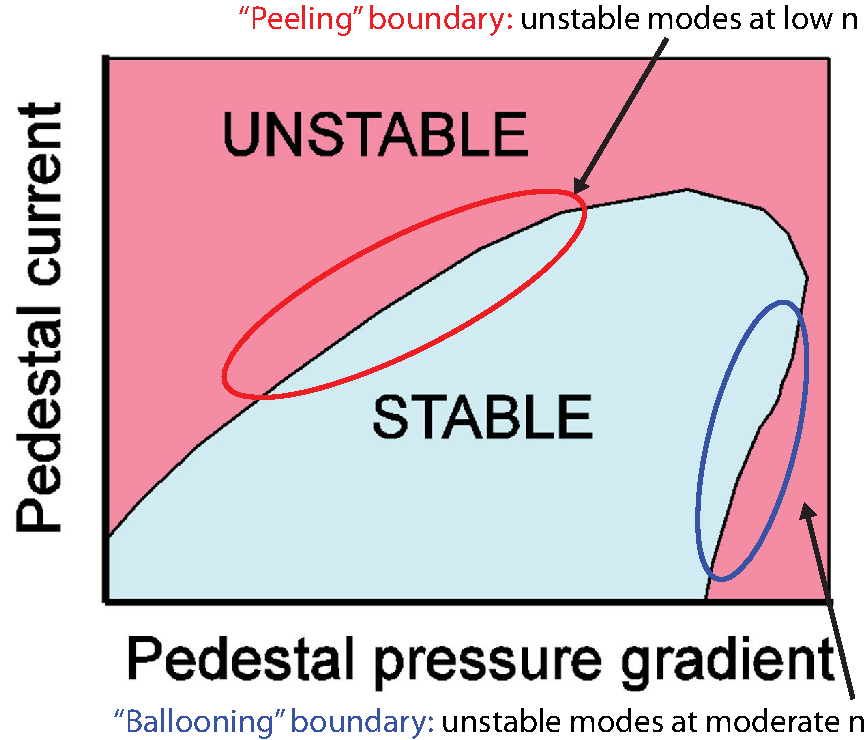
\includegraphics[width=100mm]{graphics/ModelingTheory/pbcartoon.pdf}}
\end{figure}

\begin{figure}
 \pushtooutside
 \fcapside[60mm]{\caption[ELITE calculation of P-B stability in a C-Mod ELMy H-mode.]{Calculation of the peeling-ballooning MHD stability contour from ELITE for an ELMy H-mode pedestal on C-Mod.  To within error bars, the pedestal lies on the peeling-ballooning boundary.  The comparatively higher collisionality typical of C-Mod H-mode pedestals pushes the MHD behavior of the pedestal towards higher-$n$, pure-ballooning modes, although moderate-$n$ coupled modes in the ``nose'' of the stability contour are also common.}\label{fig:mod_elmy_elite}}{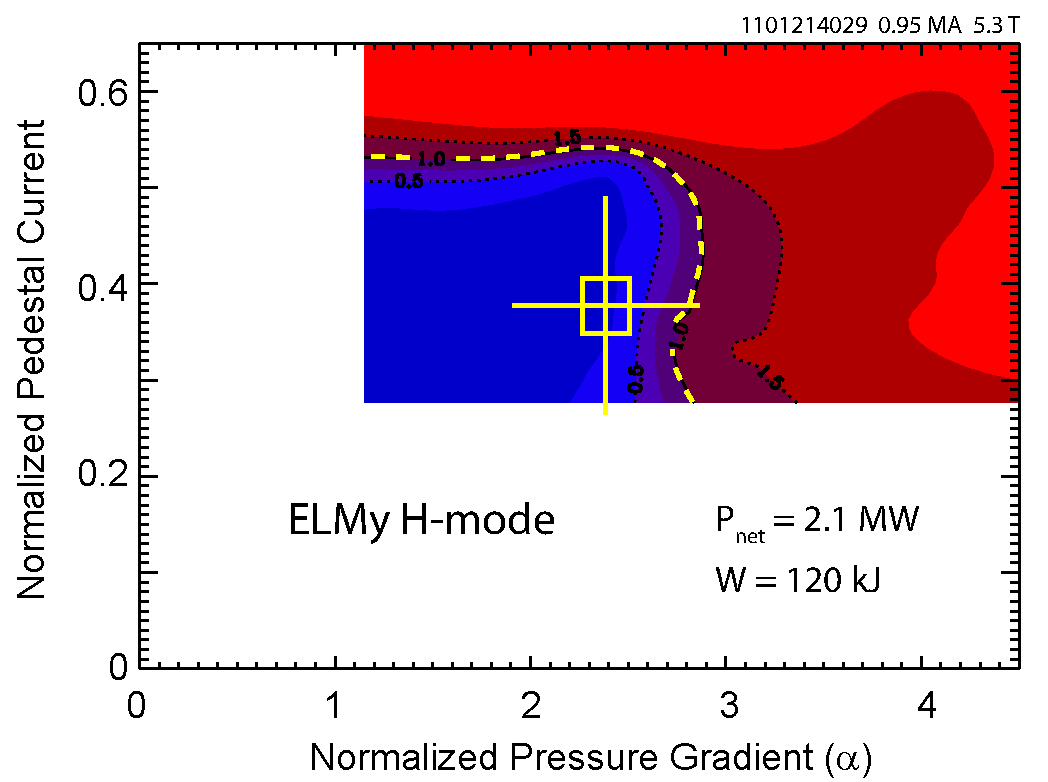
\includegraphics[width=100mm]{graphics/ModelingTheory/elmy_elite_nobal.pdf}}
\end{figure}

\nicesectionending

\section{Kinetic-Ballooning Turbulence Modeling}\label{sec:mod_turbulence}

\begin{itemize}
 \item after L-H transition, $\vec{E}\times\vec{B}$ flows continue to rise due to increased diamagnetic term $\rightarrow$ suppresses long-wavelength drift wave turbulence, drift-alfven waves.  Need short wavelength mode to limit pedestal growth. \cite{Snyder2009}
 \item ETG more likely to modify density vs. temperature, rather than limit pressure; instead consider kinetic ballooning mode \cite{Snyder2009}
 \item Snyder2009 refs Snyder thesis, Jenko2001, Scott2003, Candy2005 \cite{Snyder1999,Jenko2001,Scott2003,Candy2005}, Snyder2010 refs thesis, Jenko, Candy, add Snyder2001 \cite{Snyder2001}
 \item KBM threshold correlated to high-$n$ ideal ballooning MHD, reduced due to dissipative, ion-drift resonance effects \cite{Snyder2009}
 \item KBM onset largely independent of $\vec{E} \times \vec{B}$ shear, linear onset at $\alpha_{crit}$ \cite{Snyder2009}
 \item scaling: $\langle \alpha_c \rangle \sim \beta_{p,ped} / \Delta \rightarrow \Delta \sim \beta_{p,ped}/\langle \alpha_c \rangle$.  gradient stabilized by magnetic shear, so $\langle \alpha_c \rangle \sim 1/s^{1/2}$; $s \sim 1/j \sim 1/\beta_{p,ped} \rightarrow \alpha_c \sim \beta_{p,ped}^{1/2} \rightarrow \Delta \sim \beta_{p,ped}^{1/2}$ \cite{Snyder2009}
 \item $\beta_{p,ped}$ width scaling seen experimentally on DIII-D \cite{Osborne1998,Groebner2013}, JT-60U \cite{Oyama2005,Urano2008}, AUG \cite{Gruber1999,Beurskens2011}, C-Mod \cite{LaBombard2008,Walk2012}
 \item increased global $\beta$ increases MHD stability, but not enough to explain increased pedestal - wider pedestal with more $\beta_{p,ped}$ does explain \cite{Snyder2009a}
 \item pedestal grows maintaining $\Delta \sim \beta_{p,ped}^{1/2}$ -- KBM saturates early \cite{Maggi2010,Hughes2013}
 \item fluctuation observations of early saturation of KBM \cite{Diallo2014}
\end{itemize}

\noindent\note{BCP description!!!}

\subsection{The Ballooning-Critical Pedestal Technique}\label{subsec:mod_bcp}

The KBM is an approximately local effect due to its short scale length -- as such, no single calculated mode can describe the destabilization of the entire pedestal without a highly involved nonlocal calculation of the stability across the pedestal profile.  A far more efficient and straightforward model can be developed using the ``ballooning critical pedestal'' (BCP) technique \cite{Snyder2010,Snyder2011}, which finds the point where half of the pedestal is locally at or beyond criticality for the KBM.  At fixed pedestal width, the height is incremented to increase the pressure gradient, following the same approach as the peeling-ballooning calculation.  At each increment, the stability of the pedestal to high-$n$ ideal ballooning MHD modes is calculated, \eg using the BALOO code \cite{Connor1979,Miller1987}.  As the infinite-$n$ modes calculated by BALOO are also perfectly localized on the corresponding rational flux surfaces\gnote{explain?}, the code finds unstable surfaces in the pedestal region and the 
width of the pedestal covered by these surfaces.  When half of the pedestal width is thus unstable, the KBM threshold is said to have been reached.  This approach is highly numerically efficient -- as the ballooning MHD criterion reduces in the infinite-$n$ limit to a straightforward one-dimensional eigenvalue problem \cite{Connor1979} that can be computed efficiently -- and fairly robust, although it does require the unstable region of the pedestal to be well-defined and bounded (typically the ``middle half'' of the pedestal, where the pressure gradient is steepest).  This assumption can break down at very strong shaping or low aspect ratio \cite{Snyder2011}.\nicesectionending

\section{The EPED Model}\label{sec:mod_eped}

In light of the importance of the pedestal structure for optimized fusion performance -- both by maximizing fusion power density via the pressure pedestal height constraint on core profiles \cite{Kinsey2011}, and by avoiding or mitigating large, damaging ELMs \cite{Loarte2003,Federici2003} -- a predictive understanding of the pedestal is highly desirable for planned operations on ITER and beyond.  Models based on peeling-ballooning MHD instability, particularly the ELITE code (\cref{subsec:mod_elite}), have proven quite successful at capturing the limiting physics of the ELMy H-mode pedestal.  However, these calculations typically rely on experimental profiles and magnetic equilibria reconstructed after the fact, and as such cannot by themselves provide predictive capability.  Similarly, the constraint set by kinetic-ballooning mode (KBM) turbulence (\cref{sec:mod_turbulence}) corresponds well with pedestal observations in profiles with steep pressure gradients in the pedestal, but cannot by itself uniquely 
constrain the pedestal structure.  Here we introduce the EPED series of models \cite{Snyder2011}, which combines these two constraints into a single predictive model for the ELMy H-mode pedestal.

To incorporate predictive capability into the peeling-ballooning MHD stability model calculated by ELITE, the EPED model must characterize peeling-ballooning stability as accurately as possible using only parameters known prior to the plasma discharge, set by operator control; however, as discussed in \cref{subsec:mod_elite}, the inherent nonlocality of the problem still requires a 2-dimensional MHD calculation.  To that end, the model employs a set of model Miller equilibria \cite{Miller1998}, up/down-symmetric equilibria allowing for plasma elongation and triangularity defined with analytic plasma profiles such that the essential physics in the pedestal (namely, the pressure gradient and bootstrap current profiles) is nearly matched to experimental conditions \cite{Snyder2009}.  Using this setup, the model equilibria may be defined by a small set of scalar parameters for use in ELITE: major and minor radius $R$ and $a$, elongation and shaping $\kappa$, $\delta$ (recall that in these up/down-symmetric 
equilibria $\delta_l = \delta_u = \delta$), plasma current $I_p$, and applied field $B_T$, set the magnetic equilibrium when combined with the target global normalized pressure (typically the Troyon normalized $\beta_N$ \cite{Troyon1984}).  Global beta also impacts the pedestal stability via the beneficial effect of increased Shafranov shift in the core on MHD stability\gnote{ref this in peeling-ballooning section!}.  The model additionally takes as inputs the density at the pedestal top $n_{e,ped}$ and the pedestal width $\Delta$ in normalized poloidal flux (note that the density and temperature profiles are defined to have the same width) to constrain the pressure and current profiles, with the current calculated from the density and temperature profiles from the analytic Sauter formula, \cref{eq:jboot} \cite{Sauter1999}.

The calculation of the peeling-ballooning stability boundary is straightforward -- at a fixed pedestal width, the pressure pedestal height (and, accordingly, the MHD instability drives from the edge pressure gradient and current density) is increased in increments until the stability boundary is reached \cite{Snyder2009}.  The interdependence between pedestal width and height is determined by repeating the calculation at a range of pedestal widths, determining a relation between the pressure pedestal width and height for a given model equilibrium.  To lowest order, the MHD limit is a limit on $\nabla p$, leading one to expect a linear relation between the pedestal width and height.  However, nonlocal effects on the MHD stability -- in particular, the broader, lower-$n$ modes destabilized by wider pedestals leading to reduced maximum $\alpha_{MHD}$ at wider $\Delta$ -- reduces the linear dependence, leading to a rough scaling of $p_{ped} \sim \Delta^{3/4}$ set by the peeling-ballooning stability boundary \
cite{Snyder2009a}.

On its own, the peeling-ballooning MHD constraint defines the pedestal height as a function of width, necessitating a second constraint to allow a unique predictive solution.  The Kinetic Ballooning Mode (KBM), described in \cref{sec:mod_turbulence}, limits the pedestal gradient with a relation $p_{ped} \sim \Delta^2$ (more precisely, $\Delta \sim \beta_{p,ped}^{1/2}$).  This constraint is sufficiently distinct from that enforced by peeling-ballooning MHD  that only a single nontrivial solution satisfying both exists -- thereby uniquely predicting the pedestal width and height.  An example of the prediction at the intersection of the P-B and KBM constraints, along with the corresponding experimental result \cite{Snyder2011}, is shown in \cref{fig:mod_epedcartoon}.

\begin{figure}[ht]
 \pushtooutside
 \fcapside[60mm]{\caption[Illustration of the peeling-ballooning MHD and KBM constraints used in the EPED model.]{Illustration of the peeling-ballooning MHD and kinetic-ballooning turbulent constraints used in the EPED model.  The peeling-ballooning constraint, calculated by ELITE, results in a trend roughly of $p_{ped} \sim \Delta_\psi^{3/4}$, while the KBM width constraint calculated via the ballooning-critical pedestal (BCP) technique sets $p_{ped} \sim \Delta_\psi^{2}$.  The unique solution to these constraints is the EPED prediction for the pedestal width and height.  The prediction is here shown compared to the measured pedestal from DIII-D shot 132003 (reproduced from \cite{Snyder2011}) \note{get permission}}\label{fig:mod_epedcartoon}}{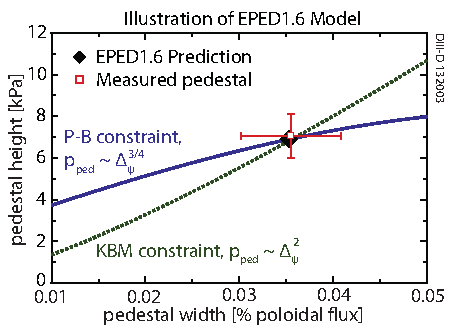
\includegraphics[width=100mm]{graphics/ModelingTheory/epedcartoon.pdf}}
\end{figure}

\subsection{EPED1}\label{subsec:mod_eped1}

The simplest version of the EPED series, EPED1 \cite{Snyder2009}, takes advantage of the dominant scaling of the width with $\beta_{p,ped}$ in the KBM constraint: as little secondary variation of the width beyond $\Delta \sim \beta_{p,ped}^{1/2}$ is seen with other expected controlling parameters, \eg $\nu^*$, $\rho^*$ or $\rho^*_{pol}$, $n_{e,ped}$ \cite{Snyder2009} (\cf \cref{sec:mod_early}, particularly \cref{subsec:mod_ionorbitloss}), the constraint is reduced to a single relation $\Delta = c \beta_{p,ped}^{1/2}$ with a fitted value for $c$.  For historical reasons based on DIII-D data, EPED1 uses $c = 0.076$, although a newer multi-machine fit produces $c = 0.084$ \cite{Snyder2011}. 

To calculate the threshold for the peeling-ballooning MHD instability, the growth rate as calculated by ELITE must be balanced against against the inherent stabilizing effect of plasma diamagnetism in the pedestal\gnote{ref or elaboration on this, or mention in ELITE section?}.  In the EPED1 model this effect is taken to be the solution to $\gamma_{MHD} = \omega (\omega - \omega_{*pi})$, where $\gamma_{MHD}$ is the instability growth rate and $\omega_{*pi}$ is the half-maximum diamagnetic frequency in the pedestal \cite{Snyder2009}.  This leads to a threshold for the growth rate of $\gamma_{MHD} > \omega_{*pi}/2$ for the peeling-ballooning onset\gnote{refs are remarkably reticent to define $\omega_{*pi}$}.  Despite this simple treatment of the KBM and P-B constraints, the EPED1 model is capable of producing predictions with a systematic $\pm 15-20\%$ uncertainty across a range of parameters \cite{Snyder2009,Snyder2010}.

\subsection{EPED1.6}\label{subsec:mod_eped16}

Although the bulk of the variation in the KBM-constrained pedestal width is captured by the $\beta_{p,ped}$ scaling, it is nevertheless desirable to account for its effects on the scale factor of the trend -- more properly, the weakly-varying function $G(\nu^*,\varepsilon,...)$ such that $\Delta = G \beta_{p,ped}^{1/2}$ -- allowing EPED to make first-principles predictions (in that the constraint is not dependent on a scale factor set by fitted data).  

The EPED1.6 implementation \cite{Snyder2010,Snyder2011} achieves this by directly calculating the KBM constraint via the ``ballooning critical pedestal'' (BCP) technique, described in \cref{subsec:mod_bcp}.    By performing this calculation across a range of pedestal widths and fitting the result against $\beta_{p,ped}$, a first-principles calculation of the KBM pedestal constraint is generated and paired with the peeling-ballooning MHD result \cite{Snyder2011}.  While this approach is more computationally expensive than the fixed scaling used in EPED1, the BCP calculation allows the effects of collisionality and shaping on the KBM threshold to be properly accounted for -- this manifests in a range of scale factors, $\langle G \rangle \approx 0.07-0.1$, that are comparable to the fitted result used in EPED1, but are specific to discharge characteristics.

The simple diamagnetic stabilization model used in EPED1, $\gamma_{MHD} > \omega_{*pi}/2$, also fails to capture important physics in the pedestal -- the model assumes a constant diamagnetic frequency $\omega_{*pi}$ for the stabilization of the peeling-ballooning modes, while in fact the diamagnetic frequency varies rapidly over the pedestal \cite{Snyder2010}.  EPED1.6 replaces this with an ``effective'' diamagnetic frequency $\omega_{*eff}$, determined by directly calculating the diamagnetic stabilization of peeling-ballooning modes in the fluid code BOUT++ \cite{Xu2010,Xia2013}.  This provides stronger stabilization of higher-$n$ ($n > \sim 12$) modes at higher collisionality than that found in the simple linear model \cite{Snyder2011,Hughes2013}, a correction that is particularly necessary for the comparatively high-collisionality pedestals in ELMy H-modes on C-Mod \cite{Hughes2013}.

\subsection{EPED Model Implementation \& ITER Predictions}\label{subsec:mod_eped_iter}

The EPED model has been extensively tested on numerous machines, particularly on DIII-D \cite{Snyder2011,Groebner2013}, JT-60U \cite{Snyder2009a}, C-Mod \cite{Walk2012}, and KSTAR \cite{Han2013}.  The model has also been tested on NSTX \cite{Groebner2013}, with limited success due to breakdown of the assumptions inherent to the KBM constraint at small aspect ratio \cite{Snyder2009a}.  Given the proximity of the pedestal to the peeling-ballooning MHD and KBM turbulence limits in most high-performance regimes, it is expected that EPED predictions are viable as a figure of merit for H-mode operation on ITER \cite{Snyder2011,Snyder2012}.

\begin{figure}[ht]
 \pushtooutside
 \fcapside[60mm]{\caption[EPED predictions versus measured pressure pedestal heights.]{EPED predictions versus measured pressure pedestal heights from DIII-D and C-Mod, spanning a significant range of pedestal pressures.  Notably, C-Mod pressure pedestals reach within a factor of $\sim 2$ of the predicted ITER pedestal height.  Reproduced from \cite{Hughes2013} \note{permission!}}\label{fig:mod_epedpredictions}}{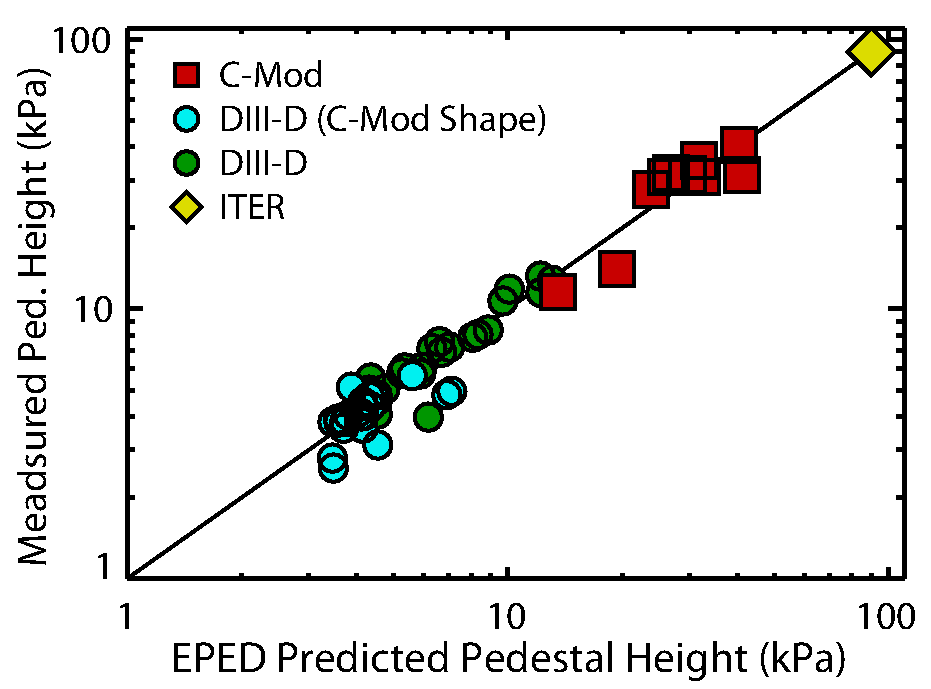
\includegraphics[width=100mm]{graphics/ModelingTheory/eped.pdf}}
\end{figure}

\noindent Notably, EPED predictions for ITER (shown compared to results from DIII-D and C-Mod \cite{Hughes2013} in \cref{fig:mod_epedpredictions}) predict pedestal pressures of $\beta_{N,ped} \sim 0.6-0.7$, corresponding to $p_{ped} \sim \SI{90}{\kilo\pascal}$, at a pedestal width of $\Delta \sim 4\%$ \cite{Snyder2009a,Snyder2011}.  This is within a factor of $\sim 2-3$ of the range of experimental results on which EPED has been tested \cite{Walk2012,Hughes2013}, and is consistent with the planned $Q=10$ operation on ITER assuming sufficient optimization of core and pedestal profiles \cite{Snyder2011,Snyder2012}.  Although development is ongoing for the EPED model series, it has demonstrated viable predictive capability for H-mode pedestals in a variety of conditions for conventional-aspect-ratio tokamaks.\nicechapterending

\bibliographystyle{../plainurl}
\bibliography{../references}